\chapter{Introduction}\label{cha:Introduction}
%All chapters should begin with an introduction before any sections begin. Further, each sections begins with an introduction before subsections begin. Chapters with just one section or sections with just one sub-section, should be avoided. Think carefully about chapter and section titles as each title stand alone in the table of contents (without associated text) and should convey meaning for the contents of the chapter or section.

%In all chapters and sections it is important to write clearly and concisely. Avoid repetitions and if needed, refer back to the original discussion or presentation. Each new section, subsection or paragraph should provide the reader with new information and be written in your own words. Avoid direct quotes. If you use direct quotes, unless the quote itself is very significant, you are conveying to the reader that you are unable to express this discussion or fact yourself. Such direct quotes also break the flow of the language (yours to someone else's).

\textit{Palynology} is the scientific study of palynomorphs, a general term for organic-walled microscopic plant and animal remains\ \parencite{askin_palynology_2003}.
Because of the resilience of these types of organisms and microfossils, the types of particles studied covers the entire geological timeline, from the earliest organisms of the Proterozoic Era, to the allergy educing grass pollens of today.

Possible applications and use cases are equally as diverse.
In criminology, soil samples can place a suspect at a specific location, depending on the composition of pollen and spores found.
Geologists analyze rock layers and use the presence and disappearance of palynomorphs to place formations in time.
Glacial Ice core samples are analyzed for organic remains to estimate temperature and rainfall over the past 10,000 years.
Finally, and most relevant to this thesis, is counting the amount of airborne pollen to forecast conditions for people suffering from allergies.

Methods used in palynology vary, but most seek to identify the composition of palynomorphs in samples taken from nature, be it from glacial ice cores, peat sections from bogs, rock samples from stratigraphic drilling, or collected airborne pollen grains.
Common for all these methods is the need for human experts to manually count and classify palynomorphs with a microscope.
A single slide can take hours to analyze and this directly affects the amount of data that can be collected and analyzed.

From a machine learning perspective, the above describes an object detection task, which is the general task of locating certain objects within an image and classifying each object.
State of the art within this problem space uses Convolutional Neural Networks (CNN), which are a type of neural network especially suited for image analysis of unprocessed image data.
However, research into the use of this technique to solve the problem of counting pollen is sparse, and as of writing only one partial example exists in literature.
Microscopy is a relatively unexplored domain for machine learning and offers unique challenges in need of research.
This thesis will therefore explore the varying methods that have been proposed to automatically count pollen grains and other similar palynomorphs, as well as other domains where modern machine learning methods have been used on similar tasks.

\section{Goals and Research Questions}\label{sec:Goals and Research Questions}
The fact that many of the major advancements within object detection have happened so recently, means that many possible use cases, pollen counting being one, have yet to be explored.
The goal of this thesis can therefore broadly be stated as follows,

\begin{description}
\item[Goal] \textit{To explore the use of Convolutional Neural Networks in automated pollen counting.}
\end{description}

The primary objective is to build a system that is able to perform the task of counting pollen grains with a accuracy comparable to that of a human expert.
Moreover than just developing a working system, the project aims to establish whether the modifications that have been successfully made to detection systems in related domains also may improve a pollen detection system.
This is formalized as the following research question,

\begin{description}
\item[RQ1] \textit{Can the computational complexity of a Single Stage MultiBox object detection model be reduced without a loss in precision and recall?}
\end{description}

Computational complexity here refers to the amount of trainable parameters that a given model is comprised of.
The Single Stage MultiBox (SSD) model is presented in Section~\ref{sec:ssd}.
It is designed as a general object detector capable of detection any number of objects in an image.
\textbf{RQ1} postulates that the task of pollen detection will require a less generalized model and that this can be realized by simplifying or removing parts of the models architecture.

Recent research in pollen classification has questioned how multifocal data may be used to improve accuracy of models operating on microscopic data, i.e.\ images from different focus planes, as opposed to single images.
This project will explore what impact the sharpness of training data has on an object detection model.
This is formalized in the second research question,

\begin{description}
    \item[RQ2] \textit{Can the accuracy and recall of the model be improved by using multifocal data?}
\end{description}

\section{Problem Description}\label{sec:back-problem}

%Pollen counting
%The Norwegian Asthma and Allergy Association has, since 1980, tracked the amount of air born pollen in Norway.
%This data is used to create a forecasting service for those who suffer allergic reactions to pollen, around 20 \% of the population.
%Pollen is collected with traps where air is continually sucked though a small slit and over an adhesive strip.
%The strip is moved across the slit, exposing different sections throughout the day.
%Pollen grains and other air born particulates adhere to the strip, which is then analyzed under a microscope.
%This produces an estimate for the density of different pollen types, measured in particles per cubic meter, throughout the season.


As mentioned, one of the primary activities within palynology is counting pollen grains.
When magnified, only a section of a slide is visible through a microscope.
A sliding window approach must be used to scan the entire surface area of the sample.
The data that is collected varies between different applications.
With airborne pollen, the slide has been prepared such that the location of the pollen represents the time interval at which it was collected.
In this case, the general location is recorded along with the taxa, such that the changes in density throughout the day are known.

\begin{figure}[htbp]
  \centering
  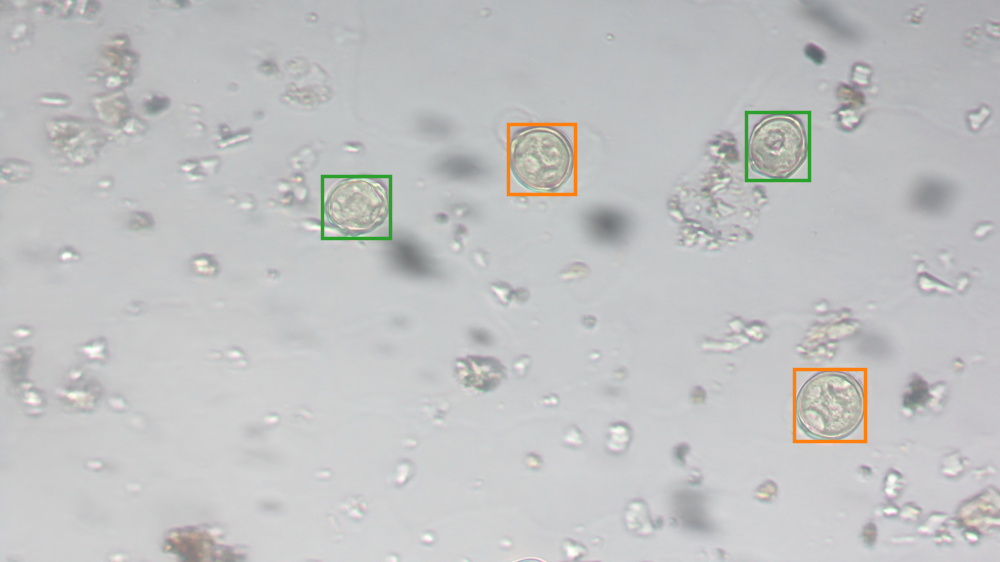
\includegraphics[width=0.7\textwidth]{figs/background/GT-Snap-080.png}
  \caption[Bounding boxes]{The image shows an LM image of 2 pollen grains with ground truth bounding boxes.
The image contains two species, \textcolor{corylus}{corylus} and \textcolor{alnus}{alnus}.}\label{fig:bbox}
\end{figure}

In the context of machine learning this can be described as an \textit{image recognition} task.
Image recognition is the general task of deciding if an image contains an object of interest, where it is located within the image, and what class the object belong to.
When the main task is to locate one or multiple objects the task is often referred to as \textit{object detection}, which is a joint regression and classification problem.
The location and dimensions of a rectangle, referred to a \textit{bounding box}, which encloses an object of interest is regressed and the object is also classified.
Figure~\ref{fig:bbox} shows a correct solution to this problem.

\section{Thesis Structure}\label{sec:intro-thesis-structure}
The remainder of this document is structured as follows,
Chapter~\ref{cha:background} covers background knowledge relating to pollen imaging techniques, the composition and functioning of Convolutional Neural Networks, and metrics for measuring performance in object detection tasks.
A literature review covering the usage of convolutional networks in object detection, as well as the various methods proposed to classify and detect pollen grains follows in Chapter~\ref{cha:related}.
Chapter~\ref{cha:method} describes the implementation and development of a CNN based object detection system, a sharpness measurement procedure, and a the experimental design used to analyze the model.
The results of these experiments are provided and discussed in Chapter~\ref{cha:results}.
